\documentclass[11pt]{scrartcl}
\usepackage{dominatrix}
\usepackage{solarized-light}
\lstset{
language=R
}
\renewcommand\thesection{Problem \arabic{section}}
\renewcommand\thesubsection{(\alph{subsection})}
\renewcommand\thesubsubsection{(\roman{subsubsection})}
\title{Homework 3}
\subject{Intro to Financial Engineering IEOR W4700}
\author{Linan Qiu\\\texttt{lq2137}}
\begin{document}
\maketitle

\section{}

\textbf{Macaulay Duration}

The price of the perpetuity $P$ is

\[P = \frac{A}{r}\]

Then, the Macaulay duration $D$ is

\[D = \frac{\sum_{i=1}^\infty i\frac{A}{(1+r)^i}}{P} = \frac{\sum_{i=1}^\infty i\frac{A}{(1+r)^i}}{\frac{A}{r}} = r\sum_{i=1}^\infty \frac{i}{(1+r)^i}\]

Now recall that

\begin{align*}
\sum_{n=1}^\infty nx^n &= x + 2x^2 + 3x^3 + ... \\
x\sum_{n=1}^\infty nx^n &= x^2 + 2x^3 + 3x^4 + ... \\
\sum_{n=1}^\infty nx^n - x\sum_{n=1}^\infty nx^n &= x + x^2 + x^3 + ... = \frac{x}{1-x} \\
\sum_{n=1}^\infty nx^n &= \frac{x}{(1-x)^2}
\end{align*}

In this case, $x = \frac{1}{1+r}$

Then,

\[D = -r \frac{\frac{1}{1+r}}{\left(1-\frac{1}{1+r}\right)^2} = -r \frac{\frac{1}{1+r}}{\frac{r^2}{(1+r)^2}} = \frac{1+r}{r}\]

\textbf{Modified Duration}

Then, the first derivative of $P$ w.r.t. $r$ is

\[\frac{dP}{dr} = -\frac{A}{r^2}\]

Then, modified duration $D_M$ is

\[D_M = - \left(-\frac{r}{A} \frac{A}{r^2}\right) = \frac{1}{r}\]

\section{}

\subsection{}

\begin{lstlisting}
> t = c(90, 91, 92, 93, 94, 95, 96, 97, 98 ,99, 100, 101)
> p = c(0.07, 0.08, 0.09, 0.1, 0.1, 0.1, 0.1, 0.1, 0.1, 0.07, 0.05, 0.04)
> crossprod(t, p)
      [,1]
[1,] 95.13
\end{lstlisting}

\[E(t) = \mathbf{t}\cdot\mathbf{p} = 95.13\]

where $\mathbf{t}$ and $\mathbf{p}$ are vectors for the age and probabilities respectively.

\subsection{}

\begin{align*}
PV(95) &= \frac{A}{r}\left(1-\frac{1}{(1-r)^5}\right) = 39927.1\\
PV(96) &= \frac{A}{r}\left(1-\frac{1}{(1-r)^6}\right) = 46228.8
\end{align*}

\begin{lstlisting}
> annuity = function(a, r, n) {(a/r)*(1-1/(1+r)^n)}
> p95 = annuity(10000, 0.08, 5)
> p96 = annuity(10000, 0.08, 6)
> p95
[1] 39927.1
> p96
[1] 46228.8
\end{lstlisting}

Then,

\[PV(95.13) = 0.13*PV(95) + 0.87*PV(96) = 45409.58\]

\subsection{}

\[E(PV) = P(90)PV(90) + P(91)PV(91) + ... + P(101)PV(101) = 38386.95\]

\texttt{annuities} is the vector $\mathbf{PV}$ while $\texttt{p}$ is the vector $\mathbf{P}$ used in the first part of the question.

\begin{lstlisting}
> n = c(0, 1, 2, 3, 4, 5, 6, 7, 8, 9, 10, 11)
> annuities = annuity(10000, 0.08, n)
> expected_annuity = crossprod(p, annuities)
> expected_annuity
         [,1]
[1,] 38386.95
\end{lstlisting}

\section{}

\subsection{}

\[P = \frac{A}{\frac{r}{12}}\left(1 - \frac{1}{(1+\frac{r}{12})^n}\right)\]

\begin{lstlisting}
> p = function(a) {(a/0.1)*(1-1/(1+0.1)^(30*12)) - 100000}
> uniroot(p, c(-999999999, 999999999))
$root
[1] 877.5716

$f.root
[1] 7.886018e-06

$iter
[1] 2

$init.it
[1] NA

$estim.prec
[1] 6.103516e-05
\end{lstlisting}

Solving for $A$ using $P=100000$ and $r=0.1$ and $n=30$ we get $A=10000$.

Total interest paid is $30*12*877.5716 - P = 215925.8$

\subsection{}

\[P = \frac{A}{\frac{r}{(26)}}\left(1-\frac{1}{\left(1+\frac{r}{(26)}\right)^{(30*26)}}\right)\]

\begin{lstlisting}
> p = function(a) {(a/(0.1/(26)))*(1-1/(1+(0.1/(26)))^(30*26)) - 100000}
> uniroot(p, c(-999999999, 999999999))
$root
[1] 404.89

$f.root
[1] 1.474004e-05

$iter
[1] 2

$init.it
[1] NA

$estim.prec
[1] 6.103516e-05
\end{lstlisting}

Solving for $A$, $A=404.89$.

Total interest paid is $30*26*404.89 - P =  215814.2$

Interest saving is $215925.8 - 215814.2 = 111.6$

\section{}

\subsection{}

Original yearly mortgage be $A$.

\[100000 = \frac{A}{0.08}\left(1 - \frac{1}{(1+0.08)^{30}}\right)\]

\begin{lstlisting}
> p = function(a){(a/0.08) * (1-1/(1+0.08)^30) - 100000}
> uniroot(p, c(-999999999, 999999999))
$root
[1] 8882.743

$f.root
[1] 1.081775e-06

$iter
[1] 2

$init.it
[1] NA

$estim.prec
[1] 6.103516e-05
\end{lstlisting}

Annual payment is $8882.743$

\subsection{}

Remaining mortgage $P$ is

\[P = \frac{A}{0.08}\left(1 - \frac{1}{(1+0.08)^{25}}\right) = 94821.29\]

\subsection{}

New yearly payment $A'$ is

\[94821.29 = \frac{A'}{0.09}\left(1 - \frac{1}{(1+0.09)^{25}}\right)\]

\begin{lstlisting}
> p = function(a){(a/0.09) * (1-1/(1+0.09)^25) - 94821.29}
> uniroot(p, c(-999999999, 999999999))
$root
[1] 9653.4

$f.root
[1] 3.295136e-07

$iter
[1] 2

$init.it
[1] NA

$estim.prec
[1] 6.103516e-05
\end{lstlisting}

$A' = 9653.4$

\subsection{}

New term $n'$ is

\[94821.29 = \frac{A}{0.08}\left(1 - \frac{1}{(1+0.08)^{n'}}\right)\]

\begin{lstlisting}
> p = function(n){(8882.743/0.09) * (1-1/(1+0.09)^n) - 94821.29}
> uniroot(p, c(-999999999, 999999999))
$root
[1] 37.56529

$f.root
[1] -0.0004005418

$iter
[1] 33

$init.it
[1] NA

$estim.prec
[1] 6.103516e-05
\end{lstlisting}

There will be $37.56529$ years remaining, which means that the total term of the mortgage is $37.56529 + 5 = 42.56529$ years.

\section{}

\subsection{}

\begin{lstlisting}
> n = c(1, 2, 3)
> discount = 1/(1+0.15)^n
> bonda = c(100, 100, 1100)
> bondb = c(50, 50, 50+1000)
> bondc = c(0, 0, 1000)
> bondd = c(1000, 0, 0)
> pricea = crossprod(discount, bonda)
> priceb = crossprod(discount, bondb)
> pricec = crossprod(discount, bondc)
> priced = crossprod(discount, bondd)
> pricea
         [,1]
[1,] 885.8387
> priceb
         [,1]
[1,] 771.6775
> pricec
         [,1]
[1,] 657.5162
> priced
         [,1]
[1,] 869.5652
\end{lstlisting}

Since yield is $0.15$, discount for each period is $\frac{1}{(1+0.15)^n}$ for each time period $n$.

Then,

\begin{align*}
P_A &= 885.8387 \\
P_B &= 771.6775 \\
P_C &= 657.5162 \\
P_D &= 869.5652
\end{align*}

\subsection{}

\[D = \frac{\sum_{i=0}^3 i * PV(i)}{P}\]

\begin{lstlisting}
> macd = function(n, bond, discount) { crossprod(n, discount*bond)/crossprod(discount, bond) }
> macd(n, bonda, discount)
         [,1]
[1,] 2.718315
> macd(n, bondb, discount)
         [,1]
[1,] 2.838321
> macd(n, bondc, discount)
     [,1]
[1,]    3
> macd(n, bondd, discount)
     [,1]
[1,]    1
\end{lstlisting}

\begin{align*}
D_A &= 2.718315 \\
D_B &= 2.838321 \\
D_C &= 3 \\
D_D &= 1
\end{align*}

\subsection{}

Sensitivity is measured by duration. C has the largest duration, hence most sensitive to yield changes.

\subsection{}

Present value $P$ of \$2,000 in 2 years is $\frac{2000}{(1+0.15)^2} = 1512.287$

\textbf{Modified duration} of this payment is

\[D_M = -\frac{1}{P}\frac{dP}{dr} = - \frac{(1+r)^2}{2000}(-2)\frac{2000}{(1+r)^3} = \frac{2}{1+r} = \frac{2}{1 + 0.15} = 1.73913\]

The two equations are:

\begin{align*}
V_A + V_B + V_C + V_D &= 1512.287 \\
D_A V_A + D_BV_B + D_CV_C + D_DV_D &= (1.73913)(1512.287)
\end{align*}

where $D_A$ $D_B$ $D_C$ and $D_D$ are the modified durations (not the Macaulay duration calculated earlier) of each of the bonds.

If we use \textbf{Macaulay duration} instead (since the rest of the question uses Macaulay duration), then $D = 2$ for the \$2,000 payment. Then,

\begin{align*}
V_A + V_B + V_C + V_D &= 1512.287 \\
D_A V_A + D_BV_B + D_CV_C + D_DV_D &= (2)(1512.287)
\end{align*}

\subsection{}

We calculate the second derivative of each of the bond prices w.r.t yield.

\begin{lstlisting}
> p = function(r) {2000/((1+r)^2)}
> library(numDeriv)
> hessian(func=p, x=0.15)
         [,1]
[1,] 6861.039
> pricea = function(r) {100/(1+r) + 100/((1+r)^2) + 1100/((1+r)^3)}
> priceb = function(r) {50/(1+r) + 50/((1+r)^2) + 1050/((1+r)^3)}
> pricec = function(r) {0/(1+r) + 0/((1+r)^2) + 1000/((1+r)^3)}
> priced = function(r) {1000/(1+r) + 0/((1+r)^2) + 0/((1+r)^3)}
> convexa = hessian(func=pricea, x=0.15)
> convexb = hessian(func=priceb, x=0.15)
> convexc = hessian(func=pricec, x=0.15)
> convexd = hessian(func=priced, x=0.15)
> convexa
         [,1]
[1,] 7037.288
> convexb
         [,1]
[1,] 6501.704
> convexc
         [,1]
[1,] 5966.121
> convexd
         [,1]
[1,] 1315.032
\end{lstlisting}

Again, we use \textbf{Macaulay duration}. Then,

\begin{align*}
V_A + V_B + V_C + V_D &= 1512.287 \\
D_A V_A + D_BV_B + D_CV_C + D_DV_D &= (2)(1512.287)
\end{align*}

\begin{lstlisting}
> da = macd(n, bonda, discount)
> db = macd(n, bondb, discount)
> dc = macd(n, bondc, discount)
> dd = macd(n, bondd, discount)
> rhs = rbind(c(1512.287), c(2*1512.287))
> solve(rbind(c(1,1), c(da, dc)), rhs)
          [,1]
[1,]  5368.718
[2,] -3856.431
> solve(rbind(c(1,1), c(db, dc)), rhs)
          [,1]
[1,]  9353.664
[2,] -7841.377
> solve(rbind(c(1,1), c(dd, dc)), rhs)
         [,1]
[1,] 756.1435
[2,] 756.1435
\end{lstlisting}

If $V_C = 756.1435$ $V_D = 756.1435$ then we should buy 1.15 of bond C and 0.869565 of bond D.

Turns out we don't need to care about $\Gamma$ since the rest would require us to short bond C.

\subsection{}

No, since the PV of the bonds have to equal $1512.287$. However, since using bond A or B would require us to short bond C, any option that requires shorting incurs borrowing cost. If that was factored, then going pure long would be the cheapest.

At the same time, the best bond should be the one that matches the convexity of the \$2000 payment the closest. Using $\Gamma$ to denote convexity,

\[\Gamma_A V_A + \Gamma_V V_B + \Gamma_C V_C + \Gamma_D V_D \approx (6861.039)(1512.287)\]

If we add that as a third condition, we have the set of three linear equations. We can use that to find the rref, which gives us

\begin{align*}
V_A &= -26486.22 + 81.68612*t \\
V_B &= 55499.36 - 154.68809*t \\
V_C &= -27500.85 + 72.00197*t \\
V_D &= t
\end{align*}

\begin{figure}[H]
\centering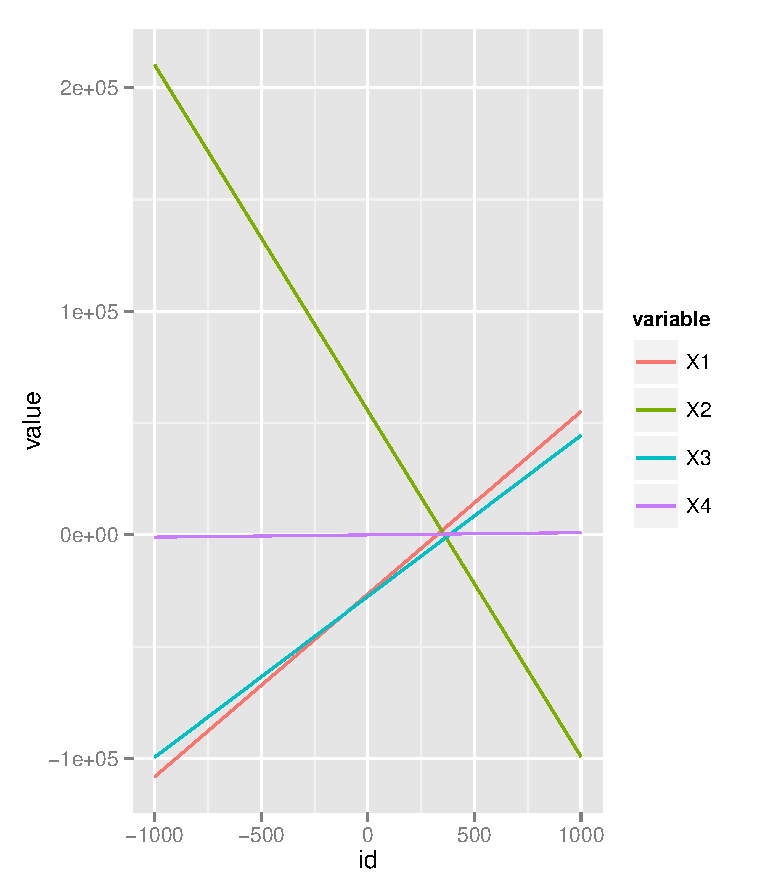
\includegraphics[width=\textwidth]{./hw3-gamma.pdf}
\caption{Plot of $V_A$ $V_B$ $V_C$ $V_D$ against $t$ where $V_D = t$. These describes values of $V_A$ $V_B$ $V_C$ $V_D$ that satisfies principal and duration hedging as well as gamma hedging. Vertical axis is the values of the 4 $V$s, and horizontal axis is the value of $t$.}
\end{figure}

\end{document}
